\documentclass{scrartcl}

\KOMAoption{toc}{bibliography}
\KOMAoptions{
	paper=a4,
	fontsize=12pt,
	parskip=true,
	titlepage=false,
	%appendixprefix=true,
	%abstract=true,
}
\addtokomafont{disposition}{\boldmath}

% section numbering
%\renewcommand*{\thesection}{\thepart.\arabic{section}}
%\DeclareTOCStyleEntry[numwidth=0.85cm]{tocline}{section}

\usepackage{fontspec}
\setmainfont{Free Serif}
\setsansfont{Free Sans}
% URLs should (still) be typed using monospace font
% https://graphicdesign.stackexchange.com/questions/97173/is-monospacing-urls-in-academic-papers-still-advised
\setmonofont{inconsolata}
%\newfontfamily\DejaSans{DejaVu Sans} % to display emojis

\usepackage{csquotes} % quotation marks
\usepackage[onehalfspacing]{setspace}
\usepackage{mathtools}
\usepackage[english,german]{translator} % siunitx needs translator package (not ngerman)! 
\usepackage{siunitx}[=v2]
\sisetup{%
	separate-uncertainty=true,
	locale=DE,
	%mode=match
	%per-mode=fraction,
}
\DeclareSIUnit\ppm{\text{ppm}}
\DeclareSIUnit\year{\text{yr}}
\NewDocumentCommand{\angsi}{omom}{%
	\ang[#1]{#2}\,\si[#3]{#4}%
}
% https://tex.stackexchange.com/questions/116426/recommend-way-to-get-angular-velocity-in-degree-with-siunitx
\usepackage[
pdfauthor={Robert Wright},
%pdftitle={},
]{hyperref}
\hypersetup{
	colorlinks=true,
	urlcolor=cyan,
	linkcolor=,
	citecolor=,
}

\usepackage{graphicx}
\usepackage[verbose]{wrapfig} % figure and text side-by-side
\usepackage{float}
\usepackage{pdfpages}
\usepackage{caption}
\usepackage{subcaption}
\usepackage[german]{cleveref}
\usepackage{booktabs, makecell}
\usepackage[roman]{parnotes}
\usepackage[shortcuts]{extdash} % to hyphenate words with dashes in them
\usepackage{xcolor}
\usepackage[enable]{easy-todo}
\usepackage[version=4]{mhchem}

% LANGUAGE & DATE
% Note: In general, it is advisable to activate the languages
%       after all packages have been loaded
\usepackage{polyglossia}
\setdefaultlanguage{german}
%\setotherlanguages[variant=british]{english}
% load datetime2 after language is set
% (can’t detect the region with polyglossia)
\usepackage[de-DE]{datetime2}
%\DTMlangsetup[en-GB]{ord=raise}

% REFERENCES
\usepackage[
backend=biber,
style=numeric,
sorting=none,
%bibstyle=authortitle,
autolang=langname,
uniquename=init,
giveninits=true,
maxnames=2,
%block=ragged,
]{biblatex}
\addbibresource{../literature/cm1.bib}
% don't print url and urldate
%\AtEveryBibitem{
%	\clearfield{url}
%	\clearfield{urlyear}
%}

%%%%%%%%%%%%%%%%%%%%%%%%%%%%%%%%%%%%%%%%%%%%%%%%%%%%%%%%%%%%%%%%%%%%%%%%%%%%%%%%%%%
% https://tex.stackexchange.com/questions/16765/biblatex-author-year-square-brackets
\makeatletter

\newrobustcmd*{\parentexttrack}[1]{%
	\begingroup
	\blx@blxinit
	\blx@setsfcodes
	\blx@bibopenparen#1\blx@bibcloseparen
	\endgroup}

\AtEveryCite{%
	\let\parentext=\parentexttrack%
	\let\bibopenparen=\bibopenbracket%
	\let\bibcloseparen=\bibclosebracket}

\makeatother
%%%%%%%%%%%%%%%%%%%%%%%%%%%%%%%%%%%%%%%%%%%%%%%%%%%%%%%%%%%%%%%%%%%%%%%%%%%%%%%%%%%
% COSTUM COMMANDS

% change figsize globally
\newcommand{\figwidth}{0.9\linewidth}

\newcommand{\kopf}[1]{%
	\Large\textsf{\textbf{#1}}
}

% Markdown code style
\definecolor{light-gray}{gray}{0.95}
\newcommand{\code}[1]{\colorbox{light-gray}{\texttt{#1}}}

% math stuff
\newcommand*\mean[1]{\overline{#1}}
\newcommand{\vect}[1]{\boldsymbol{#1}}

% chemnistry stuff
\newcommand{\co}{\ce{CO2}}

%%%%%%%%%%%%%%%%%%%%%%%%%%%%%%%%%%%%%%%%%%%%%%%%%%%%%%%%%%%%%%%%%%%%%%%%%%%%%%%%%%%
% TITLE

\subject{Angewandte Programmierung für die Wettermodellierung}
\title{Der Einfluss von CAPE auf bodennahen Hagel in simulierten Superzellen}
\author{Robert Wright}
\publishers{Dozent: Dr. Ingo Kirchner}
\date{\DTMdisplaydate{2024}{3}{22}{-1}}

%%%%%%%%%%%%%%%%%%%%%%%%%%%%%%%%%%%%%%%%%%%%%%%%%%%%%%%%%%%%%%%%%%%%%%%%%%%%%%%%%%%

\begin{document}
	
	\maketitle
	%\tableofcontents 
	% https://tex.stackexchange.com/questions/341613/komascript-toc-prevent-column-break-between-sections-in-multicolumn-toc
	
	%\input{sections/abstract.tex}
	\section{Motivation}

% CAPE erklären
% updraft erklären
% Hagelproduktion in Gewitter anreißen und Relevanz herstellen
% Warum dieses Model?
% Meine Hypothese: Wie entsteht Hagel wo im Gewitter, warum Aufwind wichtig?

Superzellen sind bekannt für ihre Fähigkeit, enorme Mengen an Hagel zu produzieren, insbesondere große Hagelkörner mit einem Durchmesser von über \SI{4}{\cm}. Beispielsweise entstand das größte je in den USA gemessene Hagelkorn (mit einem Durchmesser von \SI{17.8}{\cm}) am 22. Juni 2003 in einer Superzelle \parencite{spektrum2003}, was ihre Gefährlichkeit verdeutlicht.

Diese Gewitterzellen zeichnen sich durch langlebige und hochreichende Mesozyklonen aus, in denen Aufwinde Geschwindigkeiten von über \SI{40}{\m\per\s} erreichen können \parencite{krider}. In diesen Aufwinden werden Wassertropfen in höhere, kältere Atmosphärenschichten transportiert, wo sie zu Eis gefrieren. Durch die Kollision mit unterkühlten Wassertropfen wächst das Hagelkorn weiter, was als Aggregation bezeichnet wird, bis es aufgrund des zunehmenden Einflusses der Schwerkraft absinkt und aus der Wolke fällt. Neben der Größe des Aufwindbereichs ist daher die maximale Vertikalgeschwindigkeit (und die entsprechende der Schwerkraft entgegengerichtete Autriebskraft) entscheidend für die Bildung großer Hagelmengen und letztere wird direkt von der Convective Available Potential Energy (CAPE) beeinflusst, auch bekannt als Labilitätsenergie. Der CAPE-Wert gibt an, wie viel Energie einem Luftpaket für den Aufstieg zur Verfügung steht und hängt unter anderem vom Feuchtegehalt der bodennahen Luftschicht ab.

Diese Analyse verändert daher indirekt das CAPE einer Atmosphäre, in welcher Superzellen simuliert werden. Anschließend wird die Vertikalgeschwindigkeit und horizontale Ausprägung der Aufwindzone quantifiziert und die Auswirkungen auf den bodennahen Hagel betrachtet.

% die Aufwinde sind viel schneller in meinen Simulationen als in echt!	
	\section{Simulationen}

Um den Einfluss von CAPE auf den Aufwind und die Produktion von Hagel in einer Superzelle zu untersuchen, wird das \textit{Cloud Model 1} (CM1), Version 20.2, \parencite{bryan2002} verwendet. Die Simulationen werden auf einem stationären Gitter der Auflösung \(\num{480}\times\num{360}\times\num{80}\) durchgeführt, dabei wird ein horizontaler Gitterpunktabstand von \SI{500}{\m} und ein vertikaler von \SI{250}{\m} gewählt. Folglich führt dies zu einem Simulationsraum von \(\SI{240}{\km}\times\SI{180}{\km}\times\SI{20}{\km}\). Der Zeitschritt beträgt \SI{1.5}{\s} und die Gesamtdauer der Simulation ist \SI{3}{\hour}, dabei werden Zwischenergebnisse alle \SI{5}{\min} abgespeichert.

\begin{table}
	\centering
	\begin{tabular}{ccS[table-format=4.1]}
		\toprule
		Label & Mischungsverhältnis [\si{\g\per\kg}] & {CAPE [\si{\J\per\kg}]} \\
		\midrule
		\texttt{MR11} & 11 & 533.5  \\
		\texttt{MR14} & 14 & 1857.7 \\
		\texttt{MR16} & 16 & 2984.9 \\
		\texttt{MR21} & 21 & 5912.5 \\
		\bottomrule
	\end{tabular}
	\caption{Durchgeführte CM1-Simulationen}
	\label{tab:sims}
\end{table}

\begin{figure}
	\centering
	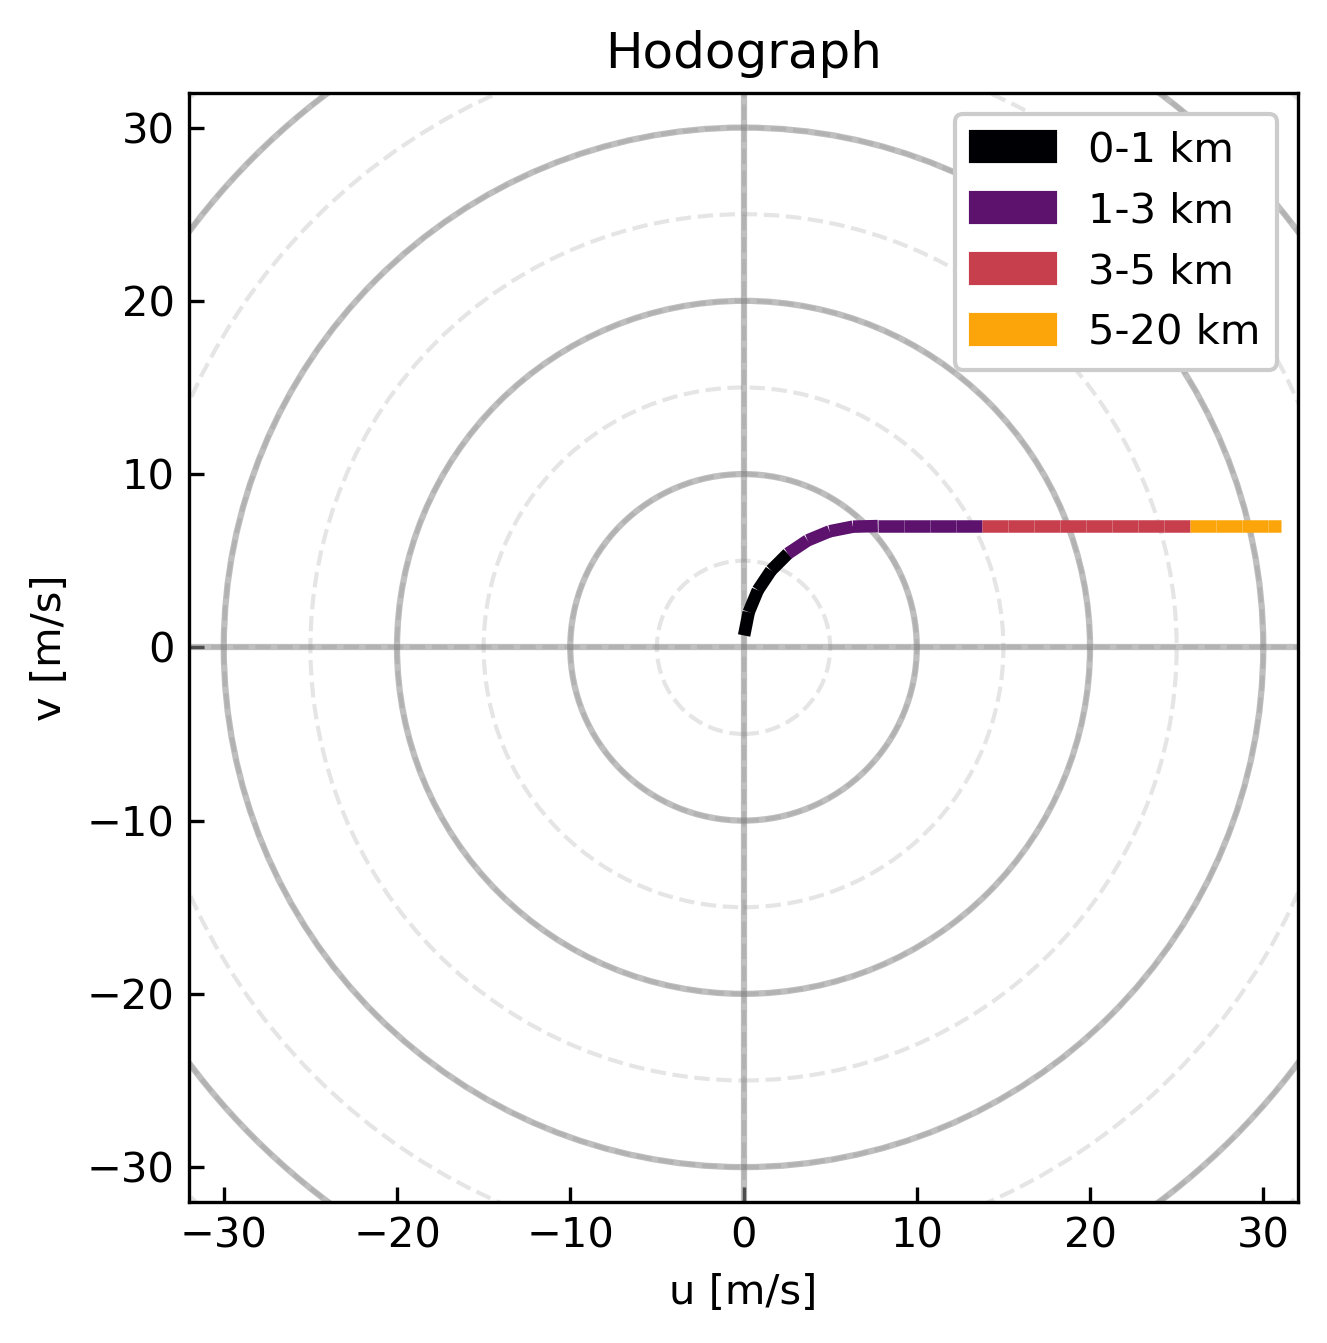
\includegraphics[width=0.6\linewidth]{../figs/hodograph.png}
	\caption{Der Hodograph zeigt die Veränderung des Windprofils mit der Höhe. Das idealisierte \textit{quarter-circle} Windprofil \parencite{weisman2000} wird in allen Simulationen unverändert verwendet.}
	\label{fig:hodograph}
\end{figure}

Die Konvektion wird durch eine Wärmeblase mit einem Temperaturunterschied von \SI{2}{\K} ausgelöst. Diese besitzt eine horizontale Ausprägung von \SI{20}{\km}, ist \SI{3}{\km} hoch und befindet sich im südwestlichen Bereich der Domain. Die Mikrophysik wird durch das \textit{two-moment Morrison scheme} \parencite{morrison2005} parametrisiert. Das Windprofil ist ein idealisierter \textit{quarter-circle} nach \textcite{weisman2000} und in \cref{fig:hodograph} dargestellt. Die Soundings der Simulationen basieren auf \textcite{weisman1982} und führen typischerweise zur Bildung von Superzellen. In den Soundings wird nun das Mischungsverhältnis von Wasserdampf zu trockener Luft erhöht (vgl. \cref{tab:sims}), was durch das niedrigere Einsetzen der Feuchtekonvektion das CAPE der Atmosphäre zu Beginn der Simulation verändert. Die gewählten Werte sind dabei aus \textcite{weisman1982} übernommen, allerdings stellt der maximale Wert des Mischungsverhältnisses \(q_v = \SI{21}{\g\per\kg}\) eine Situation dar, in der Feuchtekonvektion bereits direkt am Boden einsetzt. \(q_v\) wird dabei derart gewählt, dass bei gegebenem Umgebungsdruck und -temperatur die relative Luftfeuchtigkeit \SI{100}{\percent} beträgt. Die entsprechenden Profile sind in \cref{fig:sounding} dargestellt.

\begin{figure}
	\centering
	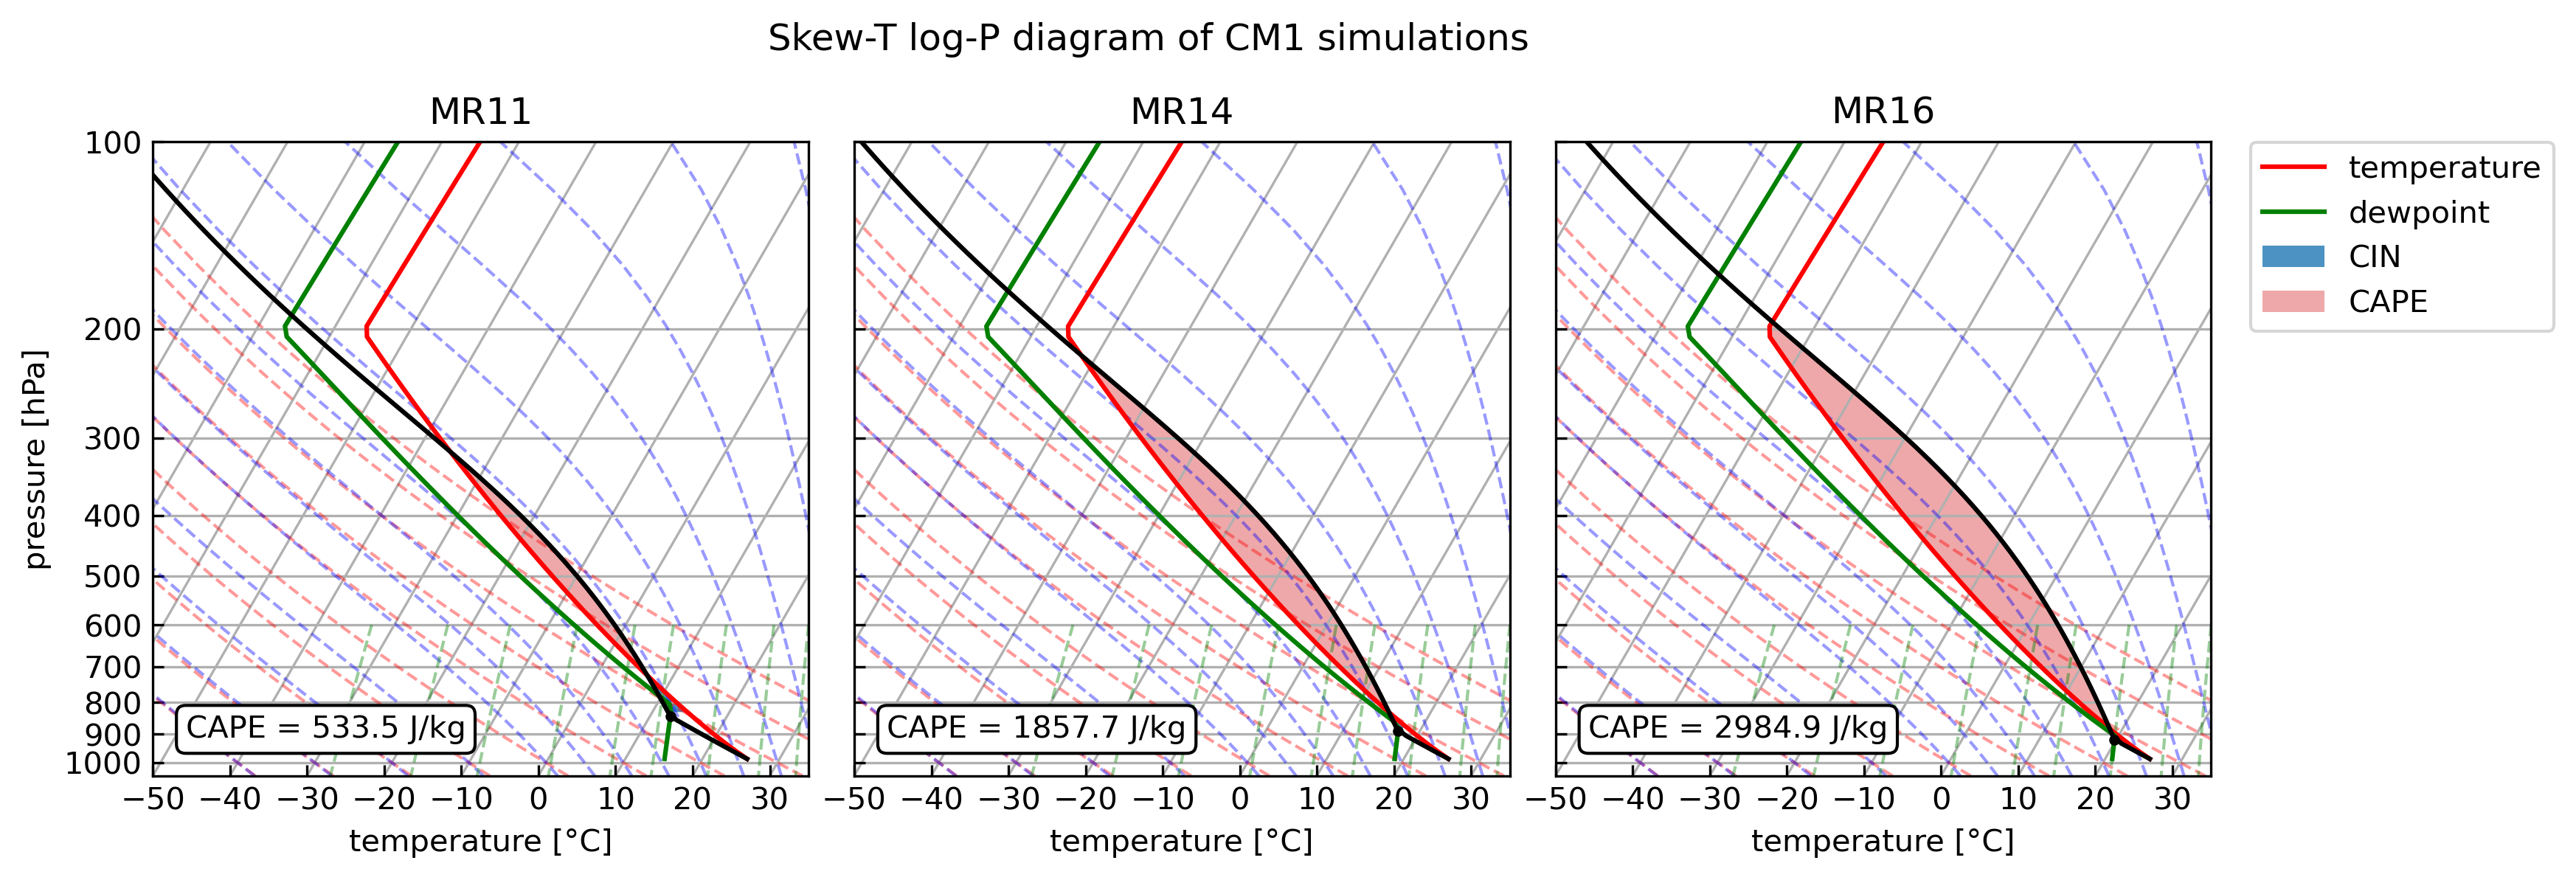
\includegraphics[width=\linewidth]{../figs/sounding.png}
	\caption{Die Soundings der einzelnen CM1-Simulationen mit vertikalem Temperatur- und Taupunktprofil. Außerdem stellt die schwarze Kurve den Aufstieg eines Luftpakets dar -- zunächst trockenadiabatisch bis zum markierten Punkt, dann setzt Feuchtekonvektion ein. Aus der Fläche zwischen Umgebungstemperatur und Temperatur des Luftpakets kann das CAPE bestimmt werden. \textit{Skew-T} betont die geneigten Isothermen.}
	\label{fig:sounding}
\end{figure}

	\section{Ergebnisse}

% Visualisierung
% reflectivity
% Vertikalgeschwindigkeit
% Hagel

Zunächst werden die Simulationen mithilfe von \textit{ParaView} visualisiert, dies dient dazu, einen Überblick über die komplexen Strukturen der Superzellen zu gewinnen und stellt sicher, dass die Ergebnisse plausibel sind und es keinen Fehler im Simulationsprozess gab. Beispielhaft wird ein Frame der Visualisierung in \cref{fig:singleframe} präsentiert, die kompletten Videos aller Simulationen sind über diesen \href{https://poincare.met.fu-berlin.de/~rw0064fu/cm1-anim/}{Link}\footnote{\hypersetup{urlcolor=}\url{https://poincare.met.fu-berlin.de/~rw0064fu/cm1-anim/}} abrufbar. Da Simulationsdaten nur alle \SI{5}{\min} zur Verfügung stehen, wird ein \textit{temporal interpolator} verwendet, allerdings sind weiterhin unschöne Sprünge zwischen den Frames erkennbar und die zeitliche Auflösung hätte weiter künstlich erhöht werden können.

\begin{figure}
	\centering
	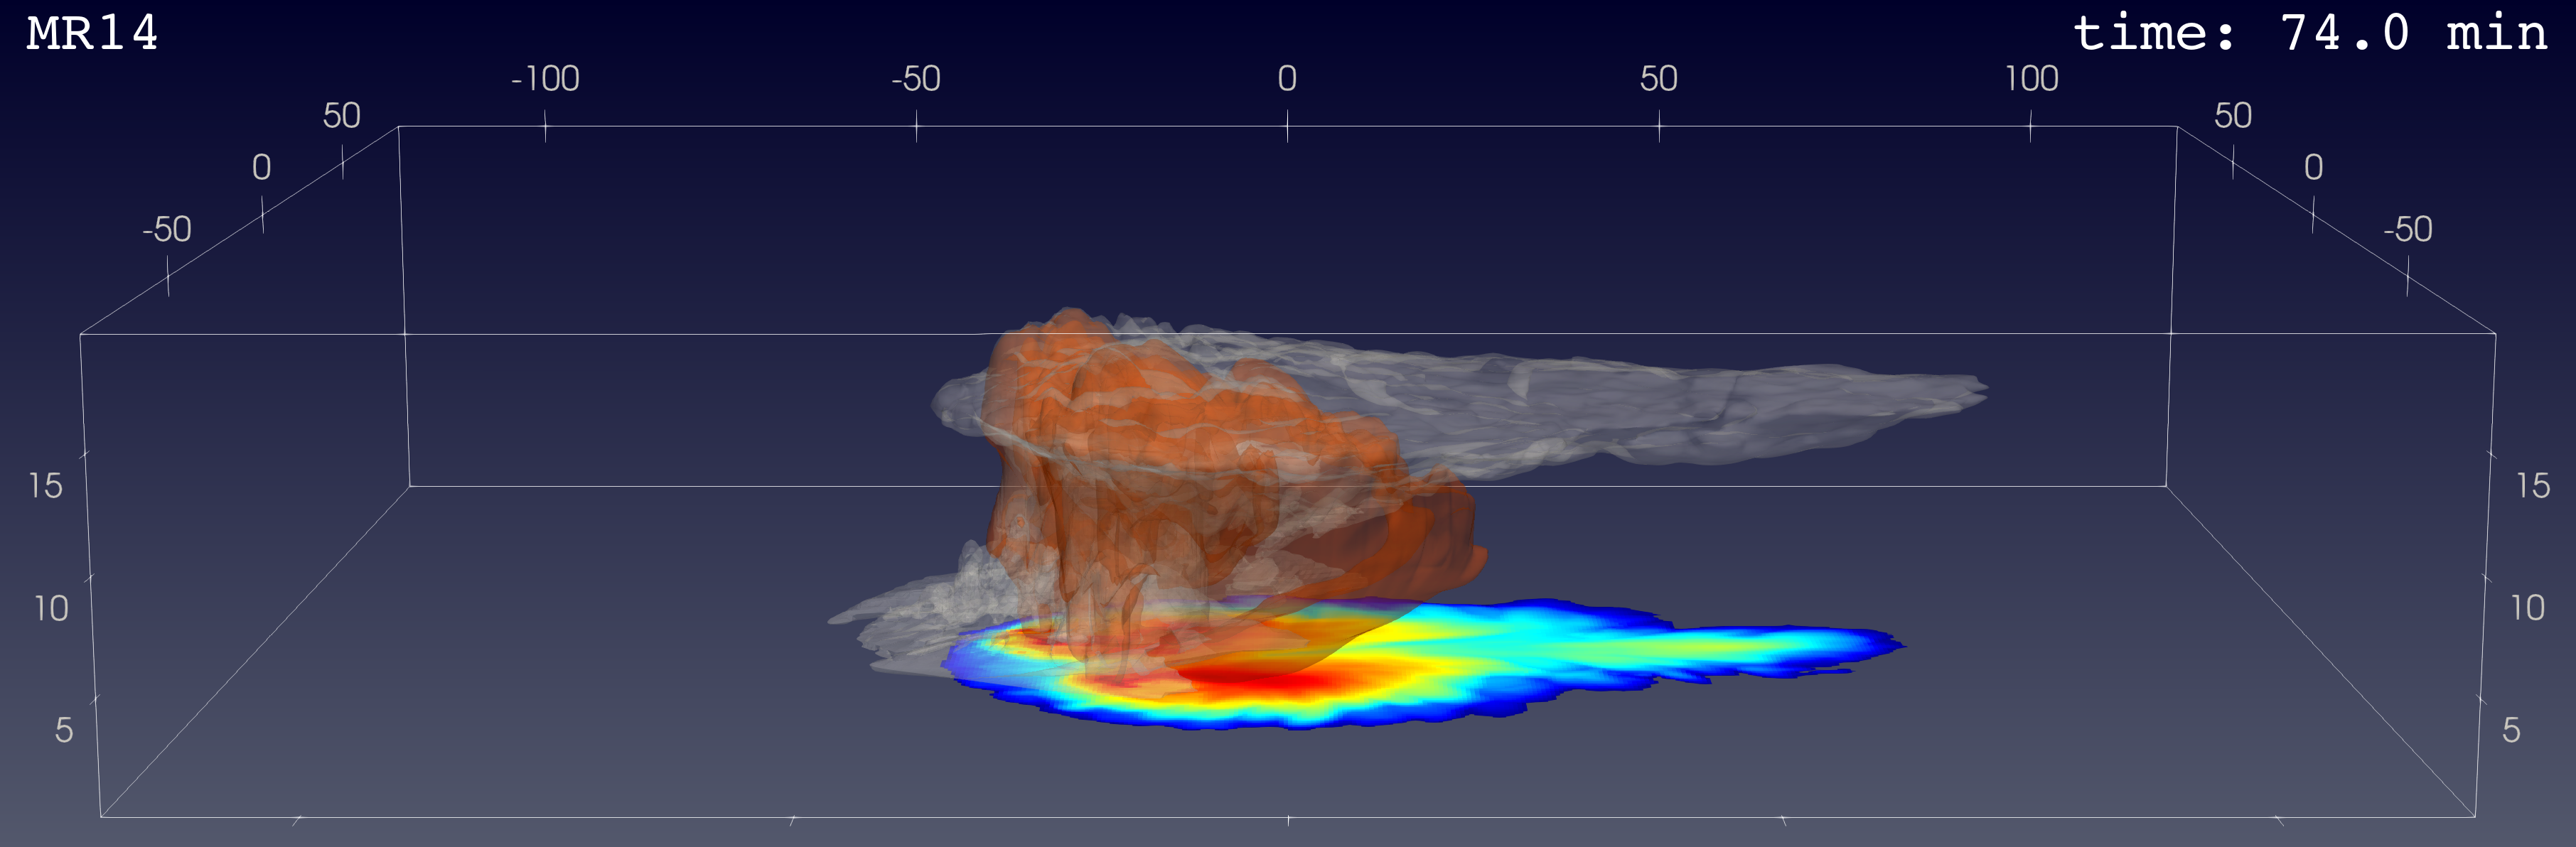
\includegraphics[width=\linewidth]{../figs/MR14-fig.0037.png}
	\caption{Die Superzelle der \texttt{MR14}-Simulation nach \SI{74}{\min} Simulationszeit. Die Konturen des Wolkenwassers sind in grau und die des Hagel-Mischungsverhältnisses in orange dargestellt. Zusätzlich ist die vertikal-integrierte maximale Reflektivität auf das niedrigste Modellniveau projiziert. Die Achsenbeschriftung gibt die Größe der Domain in \si{\km} wieder.}
	\label{fig:singleframe}
\end{figure}

In \cref{fig:cref} kann die räumliche Ausdehnung der Gewittergebilde nachvollzogen werden. In allen Simulationen ist deutlich die Aufspaltung der Superzelle in einen \textit{left-} und \textit{right-mover} zu erkennen. Dabei entstehen umso mehr lokale Gewitter entlang der Hauptpfade, je höher das Mischungsverhältnis gewählt wurde.

\begin{figure}
	\centering
	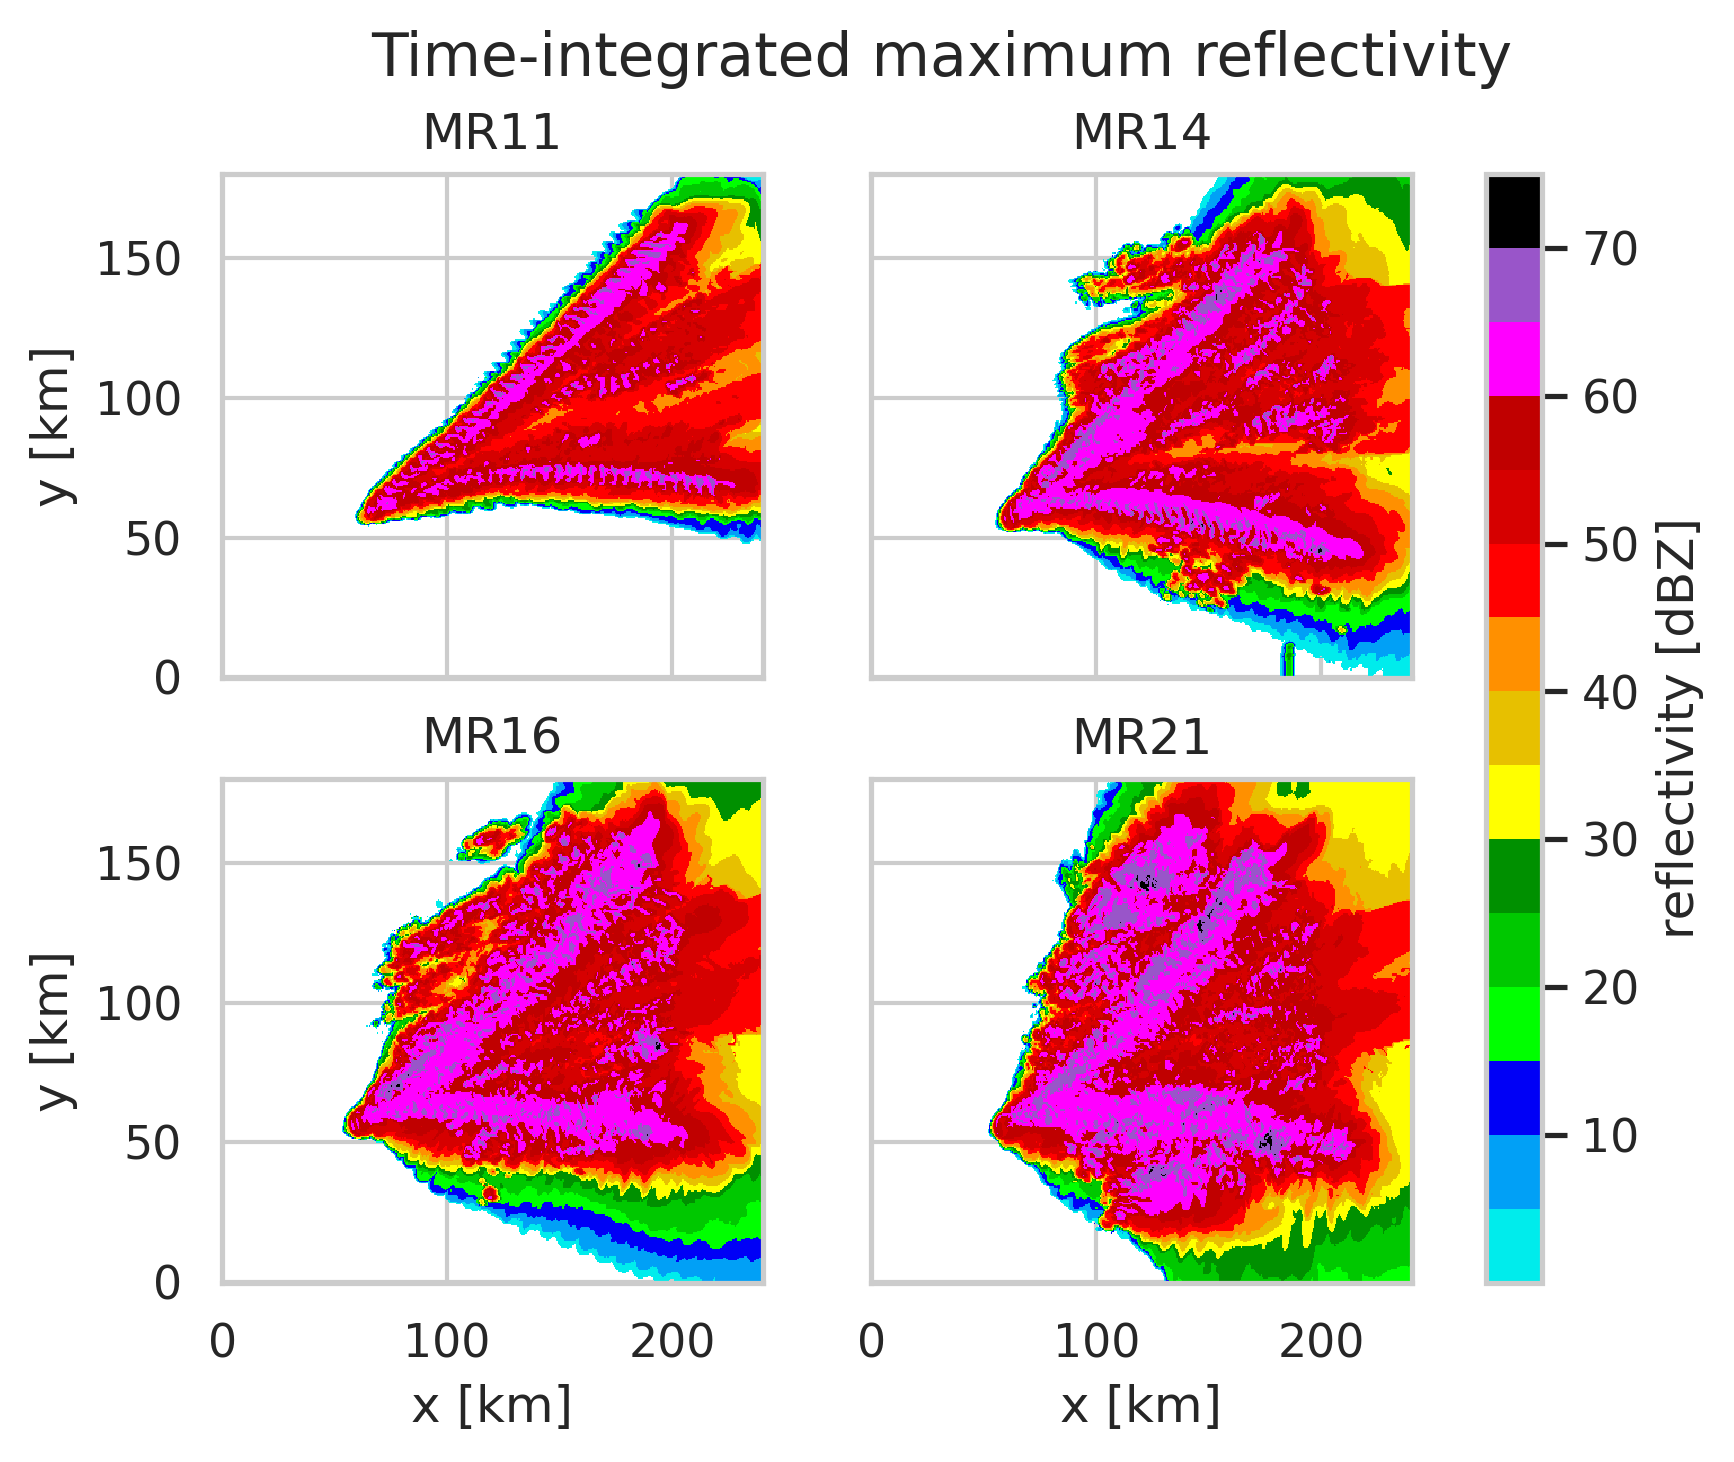
\includegraphics[width=0.8\linewidth]{../figs/cref.png}
	\caption{Die sowohl vertikal als auch zeitlich integrierte maximale Reflektivität der CM1-Simulationen}
	\label{fig:cref}
\end{figure}

Im Folgenden wird der Fokus auf die Entstehung von Hagel in den CM1-Simulationen gelegt. Daher wird der Aufwind in einer Höhe betrachtet, in der sich typischerweise Hagel bildet. Wie bereits in anderen Studien \parencite{lin2022} angenommen, wird das entsprechende Höhenintervall in dieser Analyse auf \SIrange{4}{8}{\km} AGL festgelegt. Die zeitliche Entwicklung der maximalen Vertikalgeschwindigkeit \(w\) in \cref{fig:updraft} verdeutlicht, dass eine vermehrte Verfügbarkeit von CAPE sowohl für höhere Maximalgeschwindigkeiten als auch für einen steileren Geschwindigkeitsgradienten zu Beginn der Simulation sorgt. Zur Verringerung der Maximalgeschwindigkeit bei fortgeschrittener Simulationszeit (v. a. in der \texttt{MR21}-Simulation) ist anzumerken, dass Teile des Gewittergebildes aus der Domain herauswandern. Außerdem ist der \(w \geq \SI{20}{\m\per\s}\) Aufwindbereich größer, je länger die Simulationen andauern und je höher das Mischungsverhältnis bzw. CAPE gewählt wurde.

\begin{figure}
	\centering
	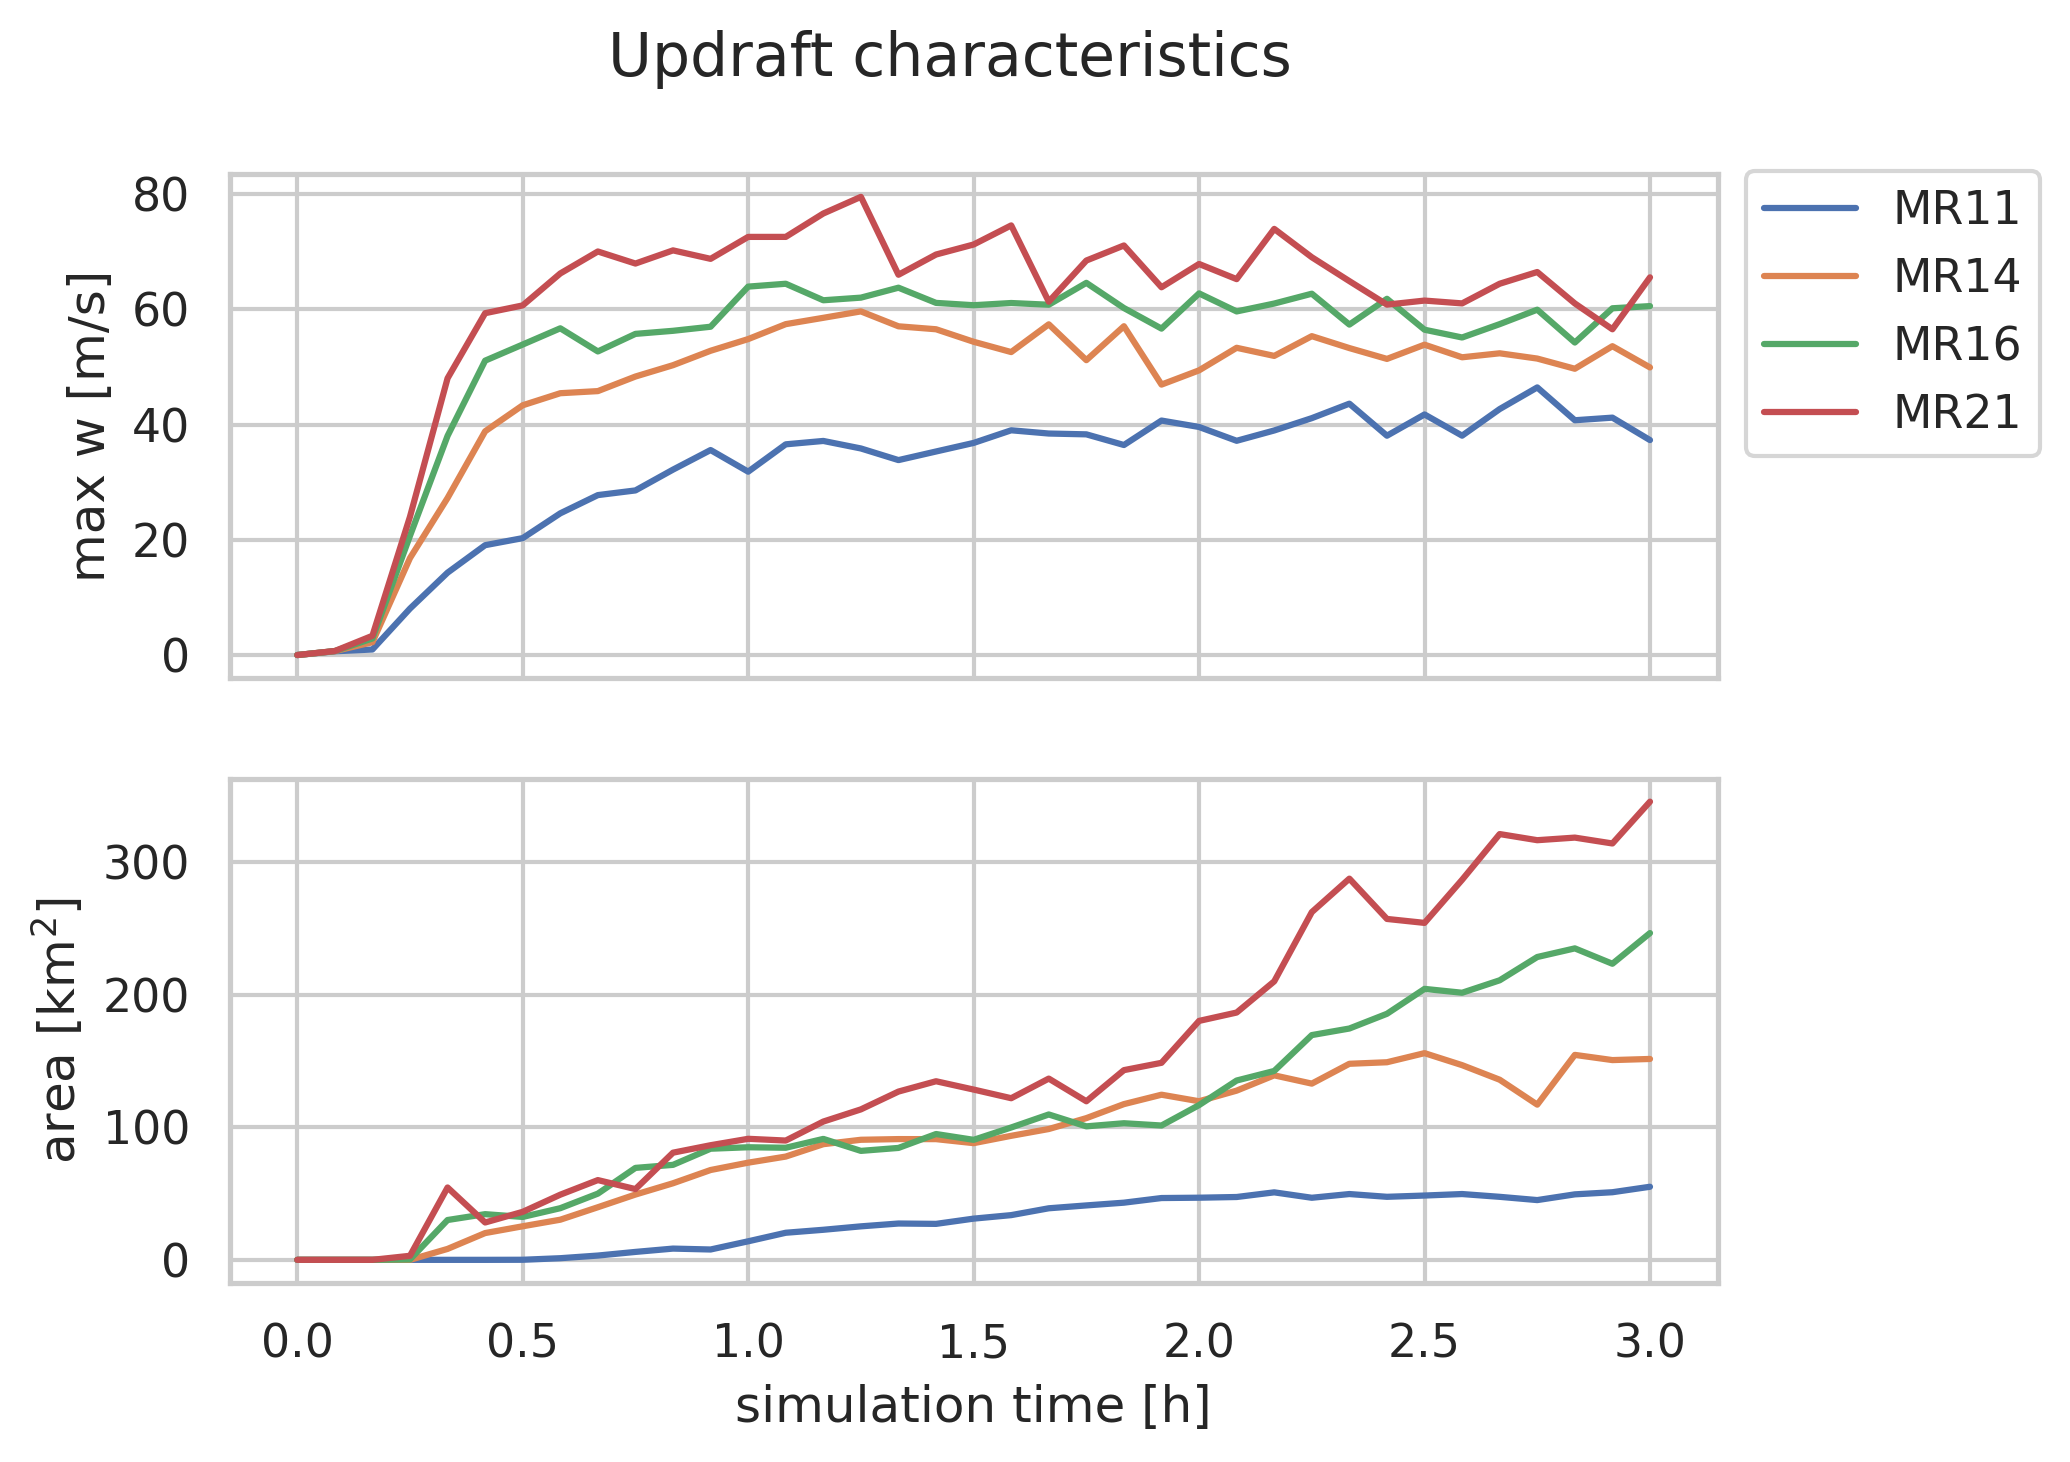
\includegraphics[width=0.9\linewidth]{../figs/updraft.png}
	\caption{\textit{Oben:} Die maximale Vertikalgeschwindigkeit des Windes über das gesamte Simulationsgebiet betrachtet. \textit{Unten:} Die gemittelte horizontale Fläche mit Aufwinden \(\geq \SI{20}{\m\per\s}\). Der Schwellenwert wurde aus \textcite{lin2022} übernommen. Beide dargestellten Größen beziehen sich auf den Bereich der optimalen Hagelentstehung zwischen \SIrange{4}{8}{\km} AGL.}
	\label{fig:updraft}
\end{figure}

Je länger die Simulationen andauern, desto mehr Hagel erreicht den Boden. Obwohl der Anstieg des Hagel-Mischungsverhältnisses \(q_h\) zunächst ähnlich zwischen den Simulationen verläuft (abgesehen von der \texttt{MR11}-Simulation, welche durchweg lediglich geringere Werte für \(q_h\) anzeigt), ändert sich dies nach ca. \SI{1.5}{\hour} Simulationszeit: Die \texttt{MR14}-Simulation erfährt eine Verringerung von \(q_h\) für etwa \SI{30}{\min}, während \texttt{MR21} ab diesem Zeitpunkt einen raschen Zuwachs an Hagel im bodennahen Bereich liefert. Darüber hinaus zeigt der rechte Subplot in \cref{fig:hail} einen Anstieg des zeitlich sowie räumlich integrierten Mittels \(\mean{q_h}\) mit zunehmendem CAPE, wobei dies für die Simulationen \texttt{MR14}-\texttt{MR21} einem linearen Zusammenhang ähnelt.

\begin{figure}
	\centering
	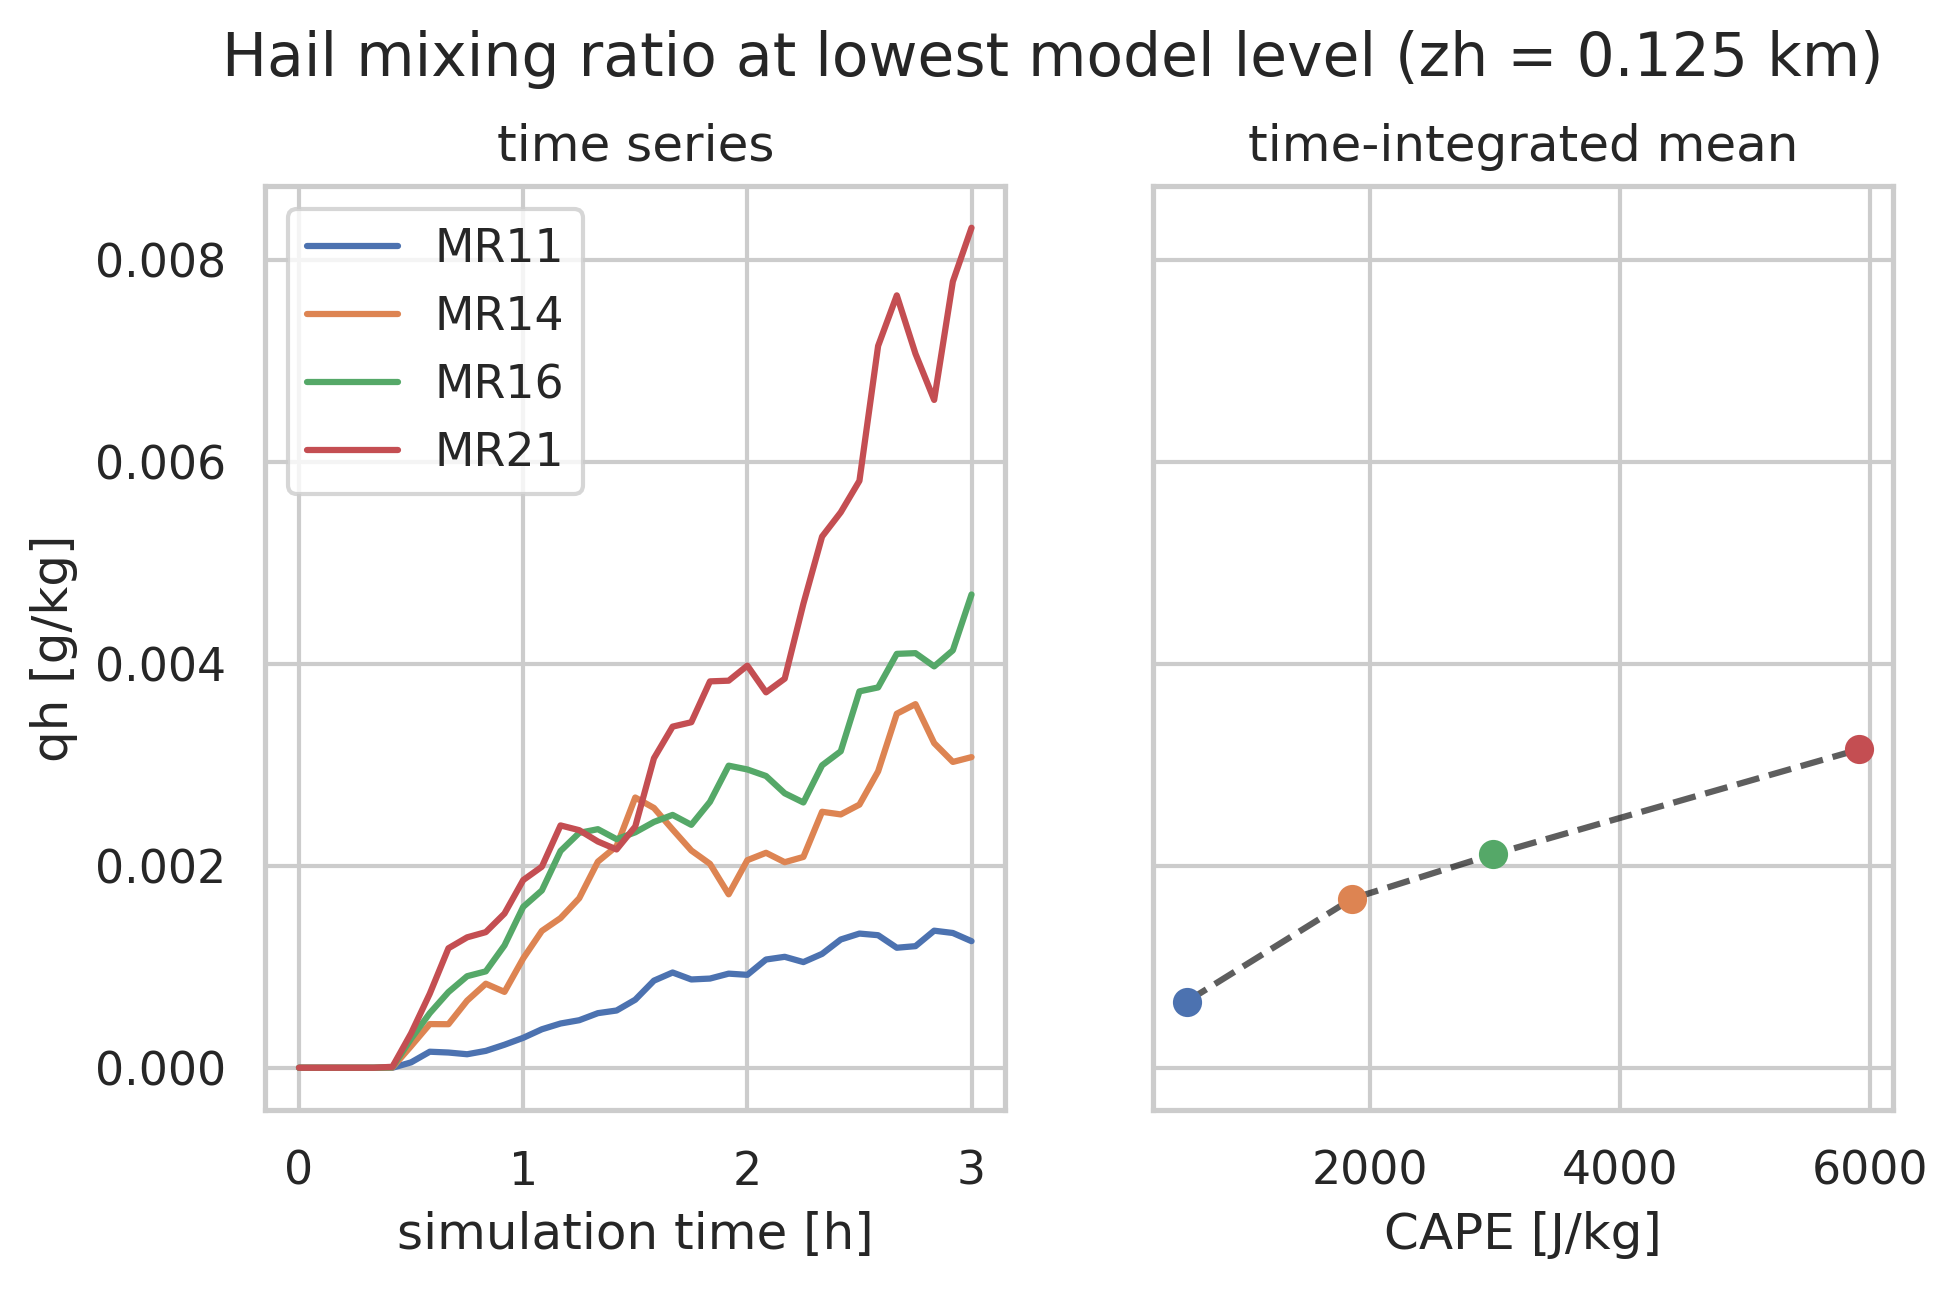
\includegraphics[width=0.9\linewidth]{../figs/hail.png}
	\caption{\textit{Links:} Die zeitliche Entwicklung des gemittelten Mischungsverhältnisses \(q_h\) von Hagel zu trockener Luft für die CM1-Simulationen. \textit{Rechts:} Das zeitliche Mittel \(\mean{q_h}\) als Funktion des CAPE. In beiden Fällen wird \(q_h\) ausschließlich auf dem niedrigsten Modellniveau berücksichtigt.}
	\label{fig:hail}
\end{figure}

Der zugrundeliegende Code dieser Analyse befindet sich auf \href{https://gitlab.met.fu-berlin.de/rw0064fu/cm1/}{GitLab}\footnote{\hypersetup{urlcolor=}\url{https://gitlab.met.fu-berlin.de/rw0064fu/cm1/}}. Einige der Abbildungen wurden mithilfe der python-Bibliothek \textit{MetPy} erstellt \parencite{may2016}.
	\section{Diskussion}

% Zunächst ist die Area gleich!

In dieser Studie wurden vier CM1-Simulationen mit unterschiedlichem Mischungsverhältnis \(q_v\) bzw. CAPE durchgeführt, um die Entstehung und insbesondere die Präsenz von Hagel im bodennahen Modellniveau zu untersuchen. In den Simulationen entstehen mehrere Superzellen, wofür vor allem das verwendete Sounding von \textcite{weisman1982} im Zusammenspiel mit der Scherung des Windes verantwortlich ist. Allerdings werden die Gewittergebilde verbreiteter, je höher das CAPE ist. Gleiches gilt für den \(w \geq \SI{20}{\m\per\s}\) Aufwindbereich, welcher zusätzlich vor allem in der zweiten Simulationshälfte deutliche Größenunterschiede zwischen den Simulationen aufweist (vgl. \cref{fig:updraft} \textit{unten}). Die erhöhten Vertikalgeschwindigkeiten bei größerem CAPE sind dagegen schon kurz nach Simulationsstart nachzuweisen (vgl. \cref{fig:updraft} \textit{oben}).

Die zeitliche Entwicklung des Hagel-Mischungsverhältnisses \(q_h\) ähnelt konzeptionell eher dem Größenverlauf des Aufwindbereichs. Diese Tatsache legt nahe, dass die höhere Menge an bodennahem Hagel auf räumlich ausgeprägtere Superzellen mit insgesamt größerer Aufwindzone zurückzuführen ist und schnellere Vertikalwinde eine untergeordnete Rolle spielen. Insgesamt bleibt jedoch festzuhalten, dass für die CM1-Simulationen mit höherem CAPE über die gesamte Simulationsdauer und Domain gemittelt mehr Hagel am Boden nachweisbar ist. Eine quantitative Analyse einzelner Aufwindschlots gleicher Fläche der unterschiedlichen Simulationen könnte die Ursache(n) für die Zunahme von \(q_h\) weiter beleuchten.
	
	\newpage
	\begingroup
	\hypersetup{urlcolor=.}
	\setlength{\emergencystretch}{3em}
	\printbibliography
	\endgroup
	
	%\newpage
	%\appendix
	%\section{Code}

Der zugrundeliegende Code dieser Analyse befindet sich auf \href{https://gitlab.met.fu-berlin.de/rw0064fu/cm1/}{GitLab}\footnote{\hypersetup{urlcolor=}\url{https://gitlab.met.fu-berlin.de/rw0064fu/cm1/}}. Einige der Abbildungen wurden mithilfe der python-Bibliothek \textit{MetPy} erstellt \parencite{may2016}.
	
\end{document}